% !TEX root = paper.tex

\vspace{4mm}
\epigraph{\textit{``Sometimes you can't see how important something is in its moment, even if it seems kind of important. This is probably one of those times.''}}{(Cyber Grand Challenge highlights from DEF CON 24, August 6, 2016)}

\vspace{-4mm}
\section{Introduction}
\label{se:intro}

%K-ICRS75
Symbolic execution is a popular program analysis technique introduced in the mid '70s to test whether certain properties can be violated by a piece of software~\cite{K-CACM76, SELECT-ICRS75,H-TSE77}. Aspects of interest could be that no division by zero is ever performed, no {\tt NULL} pointer is ever dereferenced, no backdoor exists that can bypass authentication, etc. While in general there is no automated way to decide some properties (e.g., the target of an indirect jump), heuristics and approximate analyses can prove useful in practice in a variety of settings, including mission-critical and security applications.

%While in general there is no automated way to decide some properties (think, e.g., of the halting problem), decidable approximations often exist (e.g., ``does a program always terminate within a certain amount of time?''). Such approximations can prove useful in practice in a variety of settings, including mission-critical and security applications.

In a concrete execution, a program is run on a specific input and a single control flow path is explored. Hence, in most cases concrete executions can only underapproximate the analysis of the property of interest. In contrast, symbolic execution can simultaneously explore multiple paths that a program could take under different inputs. This paves the road to sound analyses that can yield strong guarantees on the checked property. 
The key idea is to allow a program to take on {\em symbolic} -- rather than concrete -- input values. Execution is performed by a {\em symbolic execution engine}, which maintains for each explored control flow path: (i) a first-order Boolean {\em formula} that describes the conditions satisfied by the branches taken along that path, and (ii) a {\em symbolic memory store} that maps variables to symbolic expressions or values. Branch execution updates the formula, while assignments update the symbolic store. A {\em model checker}, typically based on a {\em satisfiability modulo theories} (SMT) solver~\cite{HandbookOfSAT2009}, is used to verify whether there are any violations of the property along each explored path and if the path itself is realizable, i.e., if its formula can be satisfied by some assignment of concrete values to the program's symbolic arguments.

%Variables and control flow paths are associated with expressions and constraints in terms of those symbols during a symbolic execution of the program, and constraints are eventually solved via SMT (satisfiability modulo theories) solvers.

Symbolic execution techniques have been brought to the attention of a heterogenous audience since DARPA announced in 2013 the Cyber Grand Challenge, a two-year competition seeking to create automatic systems for vulnerability detection, exploitation, and patching in near real-time~\cite{ANGR-SSP16}.
More remarkably, symbolic execution tools have been running 24/7 in the testing process of many Microsoft applications since 2008, revealing, e.g., nearly 30\% of the bugs discovered during the development of Windows 7, which other analyses and blackbox testing techniques missed~\cite{SAGE-QUEUE12}.

%In this article, we survey the main aspects of symbolic execution and discuss its extensive usage in software testing and computer security applications, where software vulnerabilities can be found by symbolically executing programs at the level of either source or binary code. We start with a simple example that highlights many of the fundamental issues addressed in the remainder of the article.

In this paper, we describe the main aspects of symbolic execution and the scalability problems it typically encounters. We discuss its extensive usage in software testing and computer security applications, where software is often available in binary form only. We start with a simple example that highlights many of the fundamental issues that arise when executing code symbolically.

% --------------------------------------------------------------------------------------------------------------------
\section{A Warm-up Example}
\label{symbolic-execution-example}

Consider the C code of Figure~\ref{fig:example-1} and assume that our goal is to determine which inputs make the  {\tt assert} at line 8 of function \texttt{foobar} fail. Since each input parameter can take as many as $2^{32}$ distinct integer values, the approach of running concretely function \texttt{foobar} on randomly generated inputs will unlikely pick up exactly the assert-failing inputs.
%Techniques such as random testing could generate bottomless input tests for this function. 
%However, it is unlikely that exactly the assert-failing inputs would be randomly picked up\mynote{Fuzzing?}. 
By evaluating the code using symbols for its inputs, instead of concrete values, symbolic execution overcomes this limitation and makes it possible to reason on {\em classes of inputs}, rather than single input values. 

\begin{figure}[t]
\begin{center}
\begin{tabular}{c}
\begin{lstlisting}[basicstyle=\ttfamily\scriptsize]
1.  void foobar(int a, int b) {
2.     int x = 1, y = 0;
3.     if (a != 0) {
4.        y = 3+x;
5.        if (b == 0)
6.           x = 2*(a+b);
7.     }
8.     assert(x-y != 0);
9.  }
\end{lstlisting}
\end{tabular}
\end{center}
\vspace{-2mm}
\caption{Warm-up example: which values of \texttt{a} and \texttt{b} make the \texttt{assert} fail?}
\label{fig:example-1}
\end{figure}

In more detail, every value that cannot be determined by a static analysis of the code, such as an actual parameter of a function or the result of a system call that reads data from a stream, is represented by a symbol $\alpha_i$. At any time, the symbolic execution engine maintains a state $(stmt,~\sigma,~\pi)$ where:

\begin{itemize}

%\item $stmt$ is the next statement to evaluate. For the time being, we assume that $stmt$ can be an assignment, a conditional branch, or a jump (more complex constructs such as function calls and loops will be discussed in  Section~\ref{se:executors} and Section~\ref{se:loops}, respectively).
\item $stmt$ is the next statement to evaluate. For the sake of simplicity, we assume that $stmt$ can be an assignment, a conditional branch, or a jump.

\item $\sigma$ is a {\em symbolic store} that associates program variables with either expressions over concrete values or symbolic values $\alpha_i$.

\item $\pi$ denotes the {\em path constraints}, i.e., is a formula that expresses a set of assumptions on the symbols $\alpha_i$ due to branches taken in the execution to reach $stmt$. At the beginning of the analysis, $\pi=true$.

\end{itemize}

\noindent Depending on $stmt$, the symbolic engine changes the state as follows:

\begin{itemize}[topsep=4pt] % TODO
  \item The evaluation of an assignment $x=e$ updates the symbolic store $\sigma$ by associating $x$ with a new symbolic expression $e_s$. We denote this association with $x\mapsto e_s$, where $e_s$ is obtained by evaluating $e$ in the context of the current execution state and  can be any expression involving unary or binary operators over symbols and concrete values.
  
%   $\alpha_i = e$: when an expression $e$ is assigned to a symbol $\alpha_i$, $pc$ is extended by adding a constraint on $\alpha_i$:
%    \[ pc \gets pc \wedge \alpha_i = e\]
%  where $e$ can be any expression, involving unary or binary operators, over symbols and constants.

  \item The evaluation of a conditional branch ${\tt if}~e~{\tt then}~s_{true}~{\tt else}~s_{false}$ affects the path constraints $\pi$. The symbolic execution is forked by creating two execution states with path constraints $\pi_{true}$ and $\pi_{false}$, respectively, which correspond to the two branches: $\pi_{true}=\pi \wedge e_s$ and $\pi_{false}=\pi \wedge \neg e_s$, where $e_s$ is a symbolic expression obtained by evaluating $e$. 
%        \[ (s_{true}, pc_{true}) \text{ where } pc_{true} = pc \wedge e \]
%        \[ (s_{false}, pc_{false}) \text{ where } pc_{false} = pc \wedge \neg e \]
    Symbolic execution proceeds independently on both states.

  \item The evaluation of a jump {\tt goto} $s$ updates the execution state by advancing the symbolic execution to statement $s$. 
\end{itemize}

\begin{figure}[t]
  \centering
  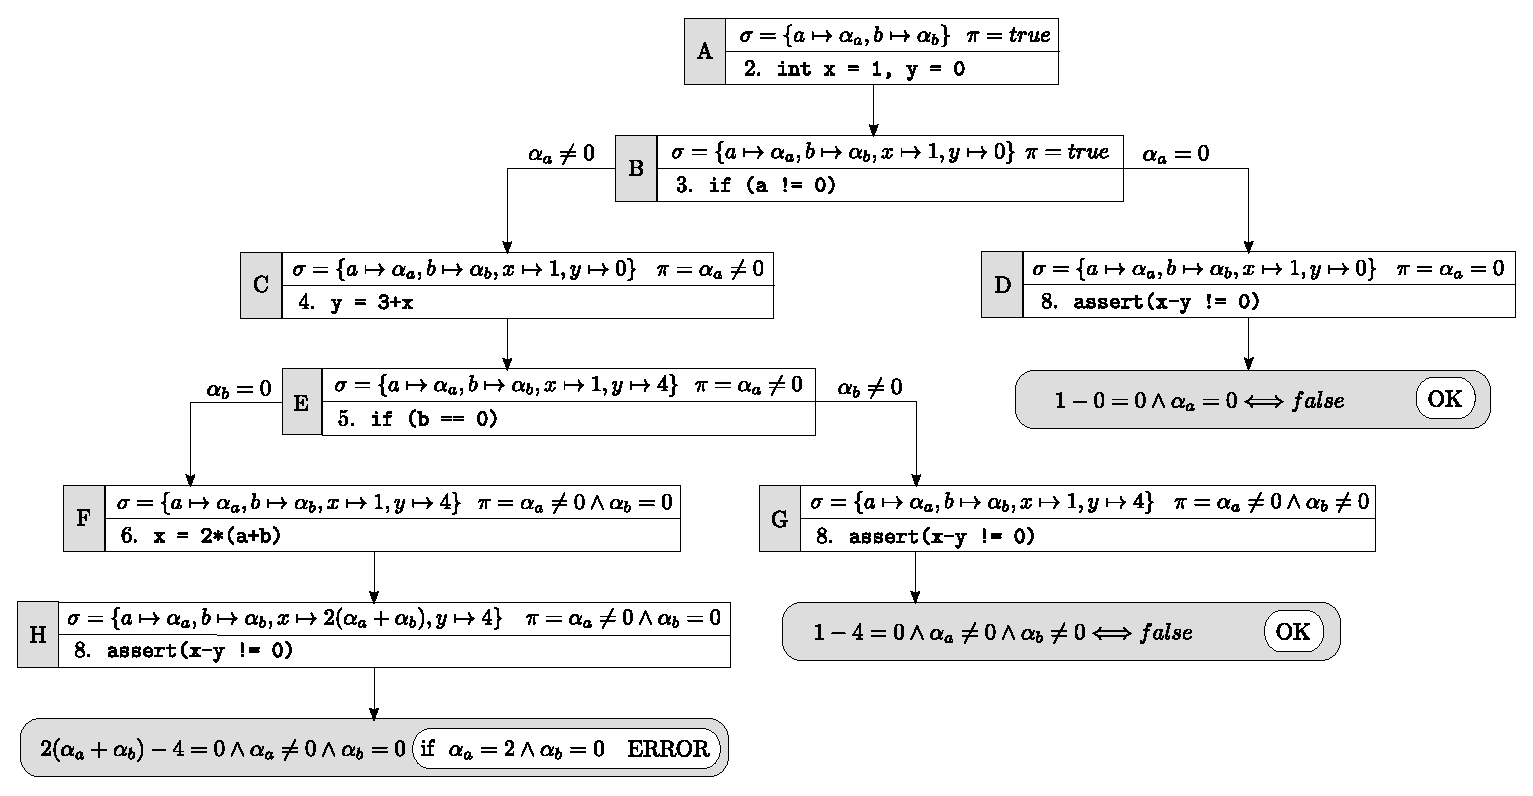
\includegraphics[width=1.0\columnwidth]{images/execution-tree.eps} 
  \caption{Symbolic execution tree of function {\tt foobar} given in Figure~\ref{fig:example-1}. Each execution state, labeled with an upper case letter, shows the statement to be executed, the symbolic store $\sigma$, and the path constraints $\pi$. Leaves are evaluated against the condition in the {\tt assert} statement. }
%For the sake of presentation the conjunction of constraints is shown as a list of constraints. }
  \label{fig:example-symbolic-execution}
\end{figure}

\noindent A symbolic execution of function {\tt foobar}, which can be effectively represented as a tree, is shown in Figure~\ref{fig:example-symbolic-execution}. Initially (execution state $A$) the path constraints are {\tt true} and input arguments {\tt a} and {\tt b} are associated with symbolic values. 
After initializing local variables {\tt x} and {\tt y} at line 2, the symbolic store is updated by associating {\tt x} and {\tt y} with concrete values 1 and 0, respectively (execution state $B$). Line 3 contains a conditional branch and the execution is forked: depending on the branch taken, a different statement is evaluated next and different assumptions are made on symbol $\alpha_a$ (execution states $C$ and $D$, respectively). In the branch where $\alpha_a\neq 0$, variable {\tt y} is assigned with ${\tt x}+3$, obtaining $y\mapsto 4$ in state $E$ because $x\mapsto 1$ in state $C$. In general, arithmetic expression evaluation simply manipulates the symbolic values.
After expanding every execution state until the {\tt assert} at line 8 is reached on all branches, we can check which input values for parameters {\tt a} and {\tt b} can make the {\tt assert} fail. By analyzing execution states $\{D,G,H\}$, we can conclude that only $H$ can make {\tt x-y = 0} true. The path constraints for $H$ at this point implicitly define the set of inputs that are unsafe for {\tt foobar}. 
In particular, any input values such that:
 \[ 2(\alpha_a+\alpha_b)-4 = 0 \wedge \alpha_a \neq 0 \wedge \alpha_b = 0 \]
will make {\tt assert} fail. An instance of unsafe input parameters can be eventually determined by invoking a {\em model checker}~\cite{HandbookOfSAT2009} to solve the path constraints, which in this example would yield $a = 2$ and $b = 0$. 

%Notice\mynote{Say earlier?} that a constraint solver is also needed when evaluating the satisfiability of branch conditions.

% --------------------------------------------------------------------------------------------------------------------
\section{Challenges in Symbolic Execution}
\label{example-discussion}

In the example discussed in Section~\ref{symbolic-execution-example} symbolic execution can identify {\em all} the possible unsafe inputs that make the {\tt assert} fail. This is achieved through an exhaustive exploration of the possible execution states. From a theoretical perspective, exhaustive symbolic execution provides a {\em sound} and {\em complete} methodology for any decidable analysis. Soundness prevents false negatives, i.e., all possible unsafe inputs are guaranteed to be found, while completeness prevents false positives, i.e.,  input values deemed as unsafe are actually unsafe. As we will discuss later on, exhaustive symbolic execution is unlikely to scale beyond small applications. Hence, in practice we often settle for less ambitious goals, e.g., by trading soundness for performance.

Challenges that symbolic execution has to face when processing real-world code can be significantly more complex than those illustrated in our warm-up example. In the remainder of this section, we address a number of observations and questions that naturally arise.

% !TEX root = main.tex


%%%%%%%%%%%%%%%%%%%%%%%%%%%%%%%%%%%%%%%%%%%%%%%%%%%%%%%%%%%
\section{Memory model}
\label{memory-model}

Our warm-up example of Section~\ref{symbolic-execution-example} presented a simplified memory model where data are stored in scalar variables only, with no indirection. A crucial aspect of symbolic execution is how memory should be modeled to support programs with pointers and arrays. This requires extending our notion of memory store by mapping not only variables, but also memory addresses to symbolic expressions or concrete values. In general, a store $\sigma$ that explicitly models memory addresses can be thought as a mapping that associates memory addresses (indexes) with either expressions over concrete values or symbolic values. We can still support variables by using their address rather than their name in the mapping. In the following, when we write $x\mapsto e$ for a variable $x$ and an expression $e$ we mean $\&x\mapsto e$, where $\&x$ is the concrete address of variable $x$. Also, if $v$ is an array and $c$ is an integer constant, by $v[c]\mapsto e$ we mean $\&v+c\mapsto e$. A memory model is an important design choice for a symbolic engine, as it can have a significant influence on the coverage achieved by symbolic execution, as well as on the scalability of constraint solving~\cite{CS-CACM13}.

The {\em symbolic memory address} problem~\cite{SAB-SP10} arises when the address referenced in the operation is a symbolic expression. In the remainder of this section, we discuss a number of popular solutions.

\subsection{Fully Symbolic Memory}
\label{ss:fully-symbolic-memory}

At the one end of the spectrum, an engine may treat memory addresses as fully symbolic. This is the approach taken by a number of works (e.g., {\sc BitBlaze}~\cite{BITBLAZE-ICISS08},~\cite{TLL-CAV10}, {\sc BAP}~\cite{BAP-CAV11}, and~\cite{TS-ATVA14}). Two fundamental approaches, pioneered by King in its seminal paper~\cite{K-CACM76}, are the following:

\begin{itemize}

\item {\em State forking.} If an operation reads from or writes to a symbolic address, the state is forked by considering all possible states that may result from the operation. The path constraints are updated accordingly for each forked state.
\boxedexample{Consider the example shown in Figure~\ref{fi:example-mem}. The write operation at line 4 affects either $a[0]$ or $a[1]$, depending on the unknown value of array index $i$. State forking creates two states after executing the memory assignment to explicitly consider both possible scenarios (Figure~\ref{fi:memory-fork}). The path constraints for the forked states encode the assumption made on the value of $i$. Similarly, the memory read operation \texttt{a[j]} at line 5 may access either $a[0]$ or $a[1]$, depending on the unknown value of array index $j$. Therefore, for each of the two possible outcomes of the assignment \texttt{a[i]=5}, there are two possible outcomes of the \texttt{assert}, which are explicitly explored by forking the corresponding states. }

\begin{figure}[ht]
\begin{center}
\begin{tabular}{c}
\begin{lstlisting}[basicstyle=\ttfamily\scriptsize]
1.  void foobar(unsigned i, unsigned j) {
2.     int a[2] = { 0 };
3.     if (i>1 || j>1) return;
4.     a[i] = 5;
5.     assert(a[j] != 5);
6.  }
\end{lstlisting}
\end{tabular}
\end{center}
\vspace{-2mm}
\caption{Memory modeling example: which values of \texttt{i} and \texttt{j} make the \texttt{assert} fail?}
\label{fi:example-mem}
\end{figure}

\begin{figure}[ht]
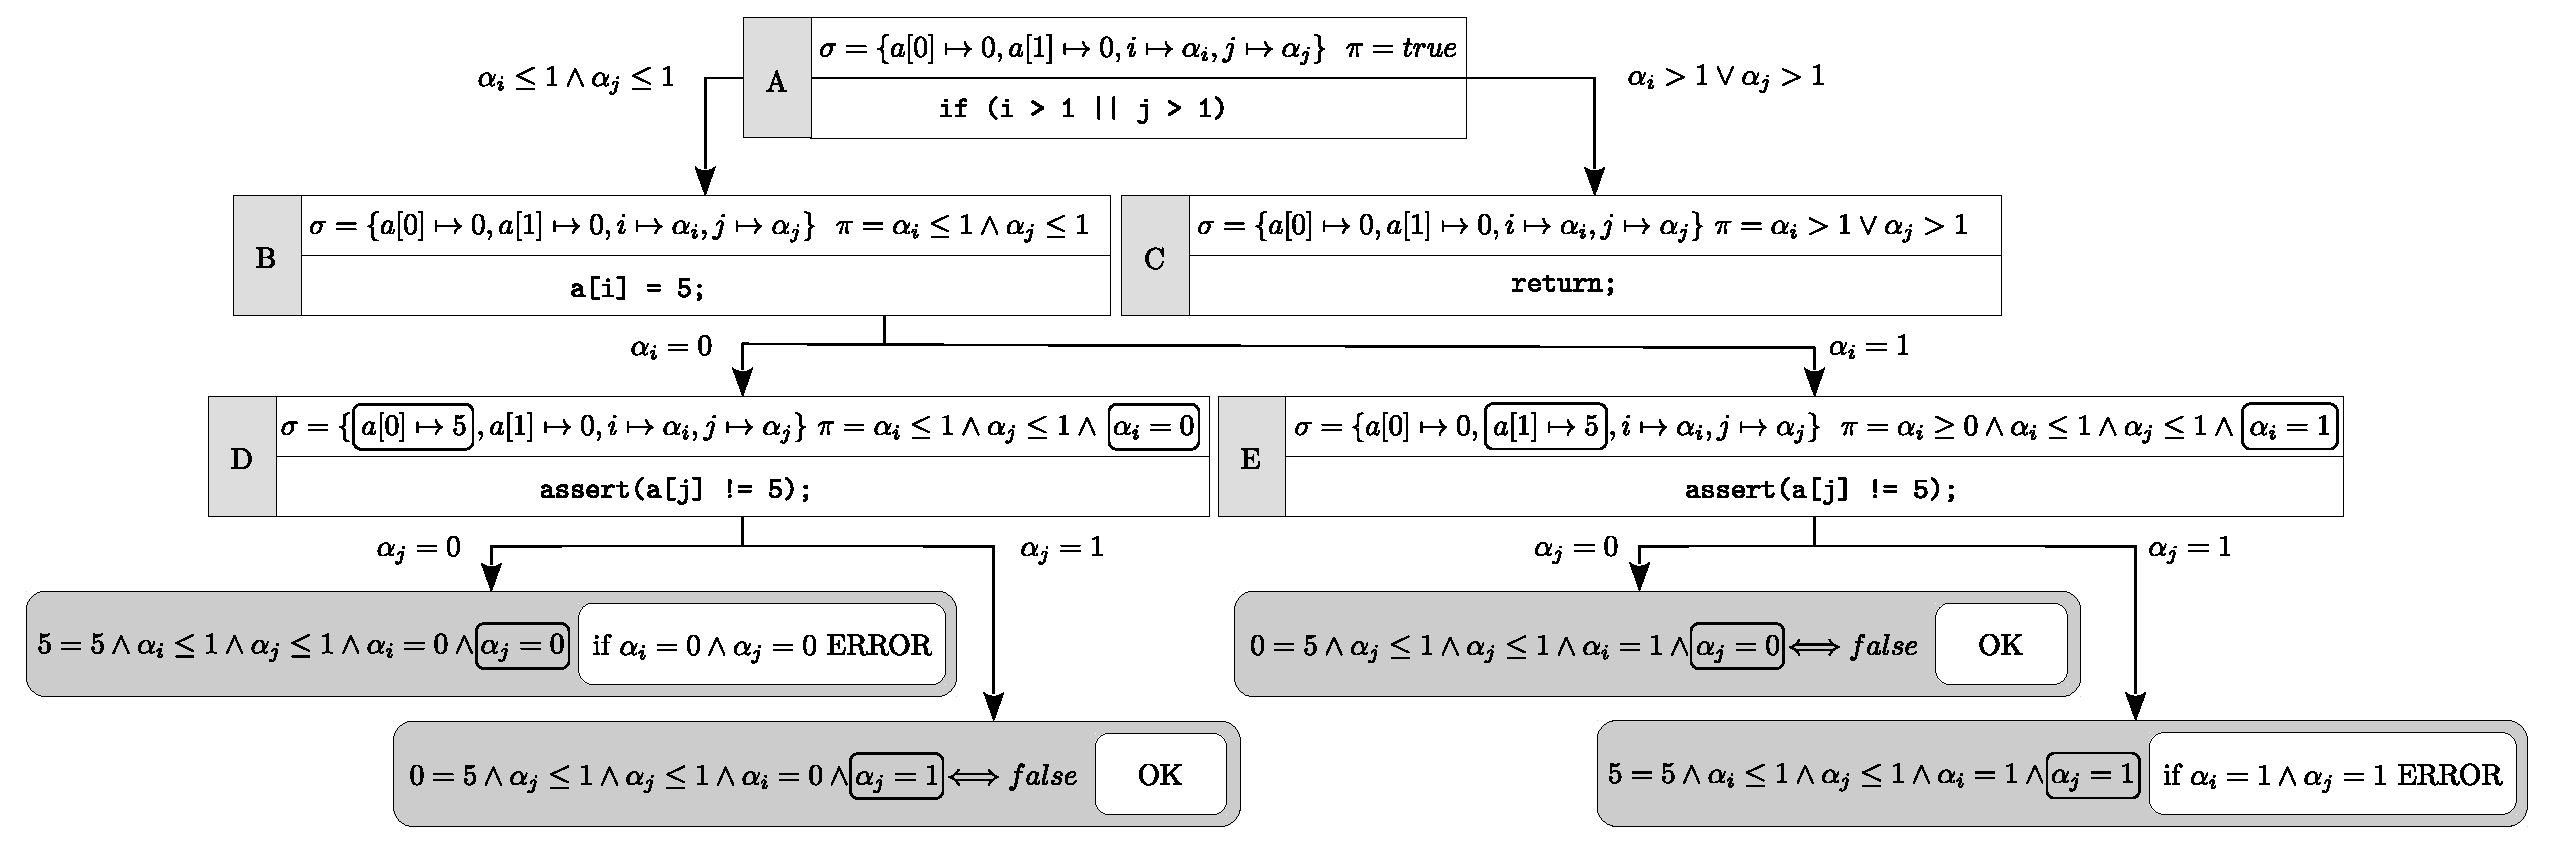
\includegraphics[width=1\columnwidth]{images/memory-fork} 
\vspace{-4.5mm}
\caption{Fully symbolic memory via state forking for the example of Figure~\ref{fi:example-mem}.}
\label{fi:memory-fork}
\end{figure}

\item {\em if-then-else formulas.} An alternative approach consists in encoding the uncertainty on the possible values of a symbolic pointer into the expressions kept in the symbolic store and in the path constraints, without forking any new states. The key idea is to exploit the capability of some solvers to reason on formulas that contain if-then-else expressions of the form $ite(\texttt{c}, \texttt{t}, \texttt{f})$, which yields \texttt{t} if \texttt{c} is true, and \texttt{f} otherwise\footnote{In propositional logic, the $ite(\texttt{c}, \texttt{t}, \texttt{f})$ expression could be replaced with the formula $(\texttt{c} \wedge \texttt{t}) \vee (\neg\texttt{c} \wedge \texttt{f})$.}.
The approach works differently for memory read and write operations. Let $\alpha$ be a symbolic address that may assume the concrete values $a_1, a_2, \ldots$:
\begin{itemize}
\item reading from $\alpha$ yields the expression $ite(\alpha=a_1,\sigma(a_1), ite(\alpha=a_2,\sigma(a_2), \ldots))$;
\item writing an expression $e$ at $\alpha$ updates the symbolic store for each $a_1, a_2, \ldots$ as $\sigma(a_i)\gets ite(\alpha=a_i,e,\sigma(a_i))$.
\end{itemize}
Notice that in both cases, a memory operation introduces in the store as many $ite$ expressions as the number of possible values the accessed symbolic address may assume. The $ite$ approach to symbolic memory is used, e.g., in {\sc Angr}~\cite{ANGR-SSP16} (Section~\ref{ss:index-based-memory}).
\boxedexample{Consider again the example shown in Figure~\ref{fi:example-mem}. Rather than forking the state after the operation \texttt{a[i]=5} at line 4, the if-then-else approach updates the memory store by encoding both possible outcomes of the assignment, i.e., $a[0]\mapsto ite(\alpha_i=0,5,0)$ and $a[1]\mapsto ite(\alpha_i=1,5,0)$ (Figure~\ref{fi:memory-ite}). Similarly, rather than creating a new state for each possible distinct address of \texttt{a[j]} at line 5, the uncertainty on $j$ is encoded in the single expression $ite(\alpha_j=0,\sigma(a[0]),\sigma(a[1]))=ite(\alpha_j=0,ite(\alpha_i=0,5,0),ite(\alpha_i=1,5,0))$.
%: if $\alpha_i=0$ then $a[0]\mapsto 5$ and $a[1]\mapsto 0$; conversely, if $\alpha_i=1$ then $a[0]\mapsto 0$ and $a[1]\mapsto 5$.
%State forking creates two states after executing the memory assigment to explicitly consider both possible scenarios (Figure~\ref{fi:memory-fork}). The path constraints for the forked states encode the assumption made on the value of $i$. Similarly, the memory read operation \texttt{a[j]} at line 5 may access either $a[0]$ or $a[1]$, depending on the unknown value of array index $j$. Therefore, for each of the two possible outcomes of the assignment \texttt{a[i]=5}, there are two possible outcomes of the \texttt{assert}, which are explicitly explored by forking the corresponding states. 
}

%Indeed, the $ite(\texttt{c}, \texttt{t}, \texttt{f})$ expression introduced in the symbolic store $\sigma$ is a short term for an {\tt if-then-else} expression and means that if the condition {\tt c} is verified then {\tt t} holds, otherwise {\tt f} must be assumed as true. Nonetheless, $ite$ expressions are often just syntactic sugar for disjunctive formulas and are commonly supported by most prominent constraint solvers. For instance, in the context of propositional logic the $ite(\texttt{c}, \texttt{t}, \texttt{f})$  expression could be replaced with the formula $(\texttt{c} \wedge \texttt{t}) \vee (\neg\texttt{c} \wedge \texttt{f})$ . 

\end{itemize}

\begin{figure}[t]
\begin{center}
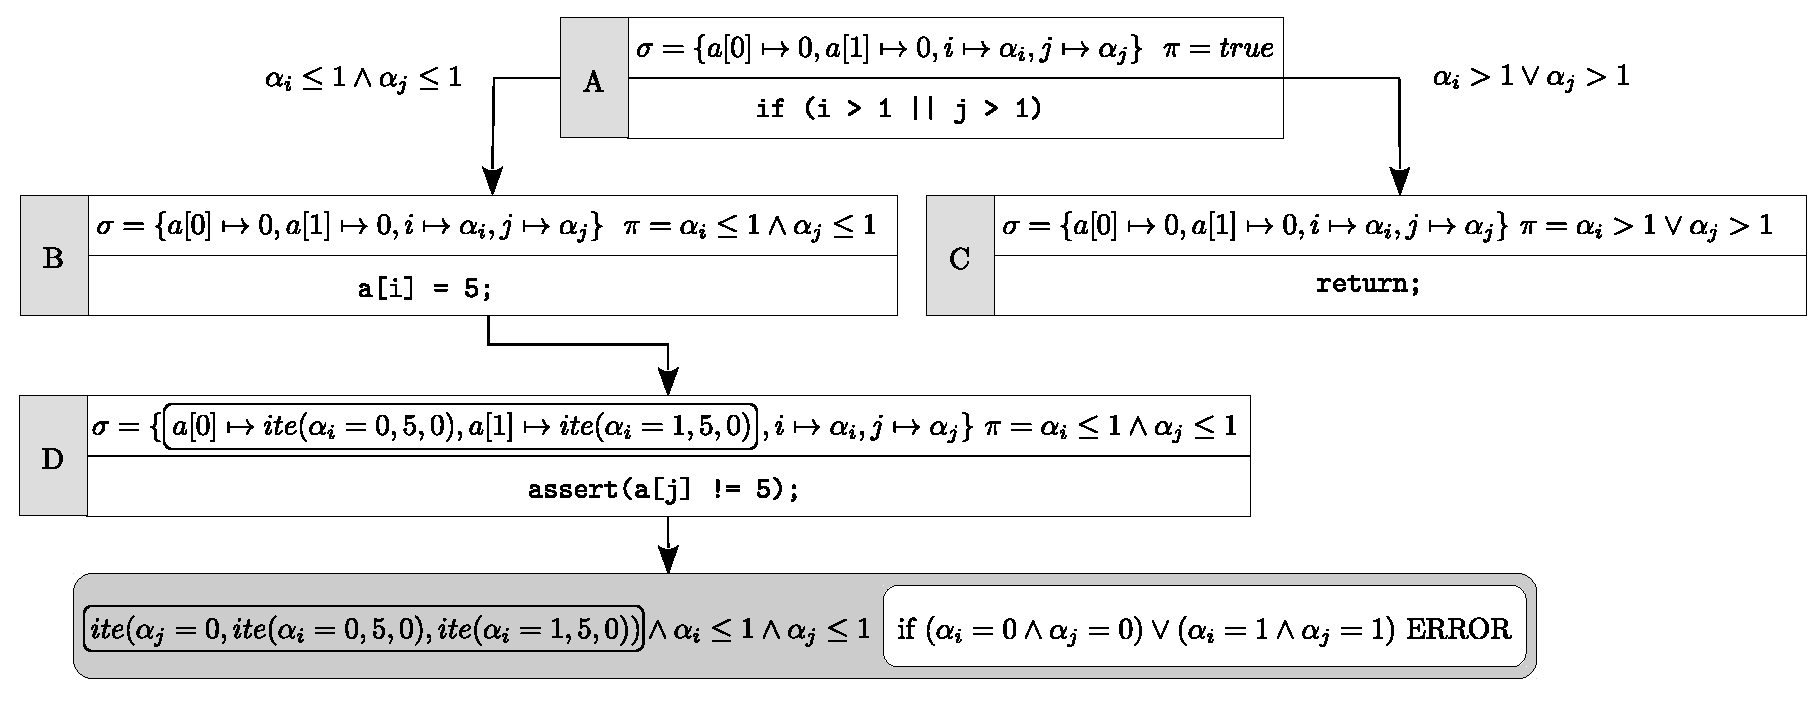
\includegraphics[width=0.7\columnwidth]{images/memory-ite} % TODO 0.7
\end{center}
\vspace{-2.5mm}
\caption{Fully symbolic memory via if-then-else formulas for the example of Figure~\ref{fi:example-mem}.}
%\vspace{-1mm} % TODO
\label{fi:memory-ite}
\end{figure}

\noindent In general, a symbolic address may reference any cell in memory, making the approaches described above intractable. Fortunately, in many practical cases the set of possible addresses a memory operation may reference is small~\cite{BITBLAZE-ICISS08}, as in the example shown in Figure~\ref{fi:example-mem} where indexes $i$ and $j$ range in a bounded interval. 

%Reasoning about all possible values a pointer may assume is notoriously hard, as in the worst case a symbolic address may reference any cell in memory. In most cases, however, symbolic memory accesses are typically already constrained to small ranges~\cite{BITBLAZE-ICISS08}. \mynote{Cite VSA \& aliasing as refinements? -- VSA is discussed below} Hence, an engine can ask the solver for the range of possible values for an address in order to restrict the exploration. 

%When obtained ranges are too large, {\sc BitBlaze}~\cite{BITBLAZE-ICISS08} adds a further constraint to the system to limit its size. However, the authors observe that most symbolic memory accesses are typically already constrained to small ranges in practice, making it unnecessary.

To model fully symbolic pointers, an extensive line of research  (e.g., {\sc EXE}~\cite{EXE-CCS06}, {\sc KLEE}~\cite{KLEE-OSDI08}, {\sc SAGE}~\cite{EGL-ISSTA09}) leverages the expressive power of some SMT solvers, which can model operations on arrays as first-class entities in constraint formulas using {\em theories of arrays} in their decision procedures~\cite{STP-CAV07}. 

%\vspace{-2pt} % TODO
\subsection{Address Concretization}
\label{ss:address-concretization}

In all cases where the combinatorial complexity of the analysis explodes as pointer values cannot be bounded to sufficiently small ranges, {\em address concretization}, which consists in concretizing a pointer to a single specific address, is a popular alternative. This can reduce the number of states and the complexity of the formulas fed to the solver and thus improve running time, although may cause the engine to miss paths that, for instance, depend on specific values for some pointers. 

%\mynote{DART is mentioned in CS-CACM13 as  using theories of arrays} --> added to the list above.
Concretization arises naturally in offline executors (Section~\ref{ss:principles}). Prominent examples are {\sc DART}~\cite{DART-PLDI05} and early {\sc SAGE} releases~\cite{SAGE-NDSS08} that concretely execute one path at a time while collecting path constraints along executed paths. %\mynote{[D] was: equality and inequality}  
Systems such as {\sc CUTE}~\cite{CUTE-FSE13} and {\sc CREST}~\cite{CREST-ASE08} are capable of reasoning only about equality constraints for pointers, as they can be solved efficiently, and resort to concretization for general symbolic references. % equality and inequality

%we normally get or set a concrete value at a particular memory address. When executing symbolically, a design choice for a symbolic engine concerns what to do when a memory reference is an expression instead of a concrete address.

%\subsection{Theory of Arrays}
%\label{ss:theory-arrays}

%A number of works (e.g., {\sc EXE}~\cite{EXE-CCS06}, {\sc KLEE}~\cite{KLEE-OSDI08}, and {\sc SAGE}~\cite{SAGE-NDSS08}) model pointers using the theory of arrays available from SMT decision procedures. 

%In this section we provide a description of its implementation in the popular STP solver~\cite{STP-CAV07}.

%The design of STP has been mainly driven by the demands of research projects on software analysis. Its input language supports one-dimensional arrays that are indexed by bitvectors and contain bitvectors. Given an array $A$, a $read(A,i)$ operation returns the value $A[i]$ at the location expressed by the index $i$, while a $write(A,i,v)$ returns a new array with the same values as $A$ at all indexes except $i$, where it contains the value $v$. Array reads and write typically appear as subexpressions of an $ite(c,a,b)$ expression, which is syntactic sugar for $(if\,c\;then\,b\;else\,a)$.

%STP reduces formulas over array to an equisatisfiable form that contains no $read$ or $write$ operations by applying three standard transformations and introducing fresh bitvector variables. Generated formulas are then amenable to SAT solving. However, transformations can also introduce bottlenecks, for instance by destroying sharing of subterms, and thus are typically procrastinated using refinement algorithms. SMT attempts also to eliminate variables through linear solving~\cite{STP-CAV07}.

%\vspace{-2pt} % TODO
\subsection{Partial Memory Modeling}
\label{ss:index-based-memory}

To mitigate the scalability problems of fully symbolic memory and the loss of soundness of memory concretization,
%Motivated by the observation that concretizing all memory indexes might not work well in some scenarios, while fully symbolic memory does not scale, 
{\sc Mayhem}~\cite{MAYHEM-SP12} explores a middle point in the spectrum by introducing a {\em partial} memory model. The key idea is that written addresses are always concretized and read addresses are modeled symbolically if the contiguous interval of possible values they may assume is small enough. This model is based on a trade-off: it uses more expressive formulas than concretization, since it encodes multiple pointer values per state, but does not attempt to encode all of them like in fully symbolic memory~\cite{MAYHEM-THESIS}. A basic approach to bound the set of possible values that an address may assume consists in trying different concrete values and checking whether they satisfy the current path constraints, excluding large portions of the address space at each trial until a tight range is found.  
%This choice is important to keep the analysis feasible: for instance, in a fully symbolic model a repeated read and write on the same symbolic index would result in quadratic increase in either the symbolic constraints or the complexity of the stored symbolic expressions~\cite{DRILLER-NDSS16}.
%Global memory is defined as a map $\mu$ from 32-bit addresses ({\em indexes}) to expressions. When a symbolic index $i$ is used to read memory, the algorithm generates a memory object $M$ containing the projection of $\mu$ over all the valid values that $i$ can assume. The evaluation of a $load(\mu,i)$ operation is thus reduced to $M[i]$, where $M$ is typically orders of magnitude smaller than the entire memory $\mu$.
%Instantiating a memory object still requires finding all the possible values for a symbolic index. A naive algorithm would employ the constraint solver to refine the range of an index using binary search under the current path constraints. 
This algorithm comes with a number of caveats: for instance, querying the solver on each symbolic dereference is expensive, the memory range may not be continuous, and the values within the memory region of a symbolic pointer might have structure. {\sc Mayhem}~\cite{MAYHEM-SP12} thus performs a number of optimizations, including Value Set Analysis~\cite{VSA-CC04} and forms of query caching (Section~\ref{se:constraint-solving}), to refine ranges efficiently. If at the end of the process the range size exceeds a given threshold (e.g., 1024), the address is concretized. {\sc Angr}~\cite{ANGR-SSP16} also adopts the partial memory model idea and extends it by optionally supporting write operations on symbolic pointers that range within small contiguous intervals (up to 128 addresses). % [D] ptr may also be redirected to symbolic data

%%%%%%%%%%%%%%%%%%%%%%%%%%%%%%%%%%%%%%%%%%%%%%%%%%%%
\subsection{Complex Objects}
\label{ss:complex-objects}

\mytempedit{\myparagraph{Lazy Initialization}}
\cite{KPV-TACAS03} propose symbolic execution techniques for advanced object-oriented language constructs, such as those offered by C++ and Java. The authors describe a framework for software verification that combines symbolic execution and model checking to handle linked data structures such as lists and trees. % [D] added dynamically allocated & discarded primitive data types, and concurrency.

In particular, they generalize symbolic execution by introducing {\em lazy initialization} to effectively handle dynamically allocated objects. Compared to our warm-up example (Section~\ref{symbolic-execution-example}), the state representation is extended with a {\em heap configuration} used to maintain such objects. Symbolic execution of a method taking complex objects as inputs starts with uninitialized fields, and assigns values to them in a lazy fashion, i.e., they are initialized when first accessed during execution.

When an uninitialized reference field is accessed, the algorithm forks the current state with three different heap configurations, in which the field is initialized with: (1) {\tt null}, (2) a reference to a new object with all symbolic attributes, and (3) a previously introduced concrete object of the desired type, respectively. This on-demand concretization enables symbolic execution of methods without the need for any previous knowledge on the number of objects given as input. Also, forking the state as in (2) results into a systematic treatment for aliasing, i.e., when an object can be accessed through multiple references.

\cite{KPV-TACAS03,SPF-ISSTA04} combine lazy initialization with user-provided {\em method preconditions}, i.e., conditions which are assumed to be true before the execution of a method. Preconditions are used to characterize those program input states in which the method is expected to behave as intended by the programmer. For instance, we expect a binary tree data structure to be acyclic and with every node - except for the root - having exactly one parent. Conservative preconditions are used to ensure that incorrect heap configurations are eliminated during initialization, speeding up the symbolic execution process.

Further refinements to lazy initialization are described in a number of works, e.g.,~\cite{DLR-ASE12,BLI-NFM13,BLISS-TSE15}, which all share the goal of reducing the number of heap configurations to generate when forking the state.~\cite{DLR-ASE12} also provides a formal treatment of lazy initialization in Java.

\mytempedit{\myparagraph{Verifying Client Code Only}}
Of a different flavor is the technique presented in~\cite{SHZ-TAIC07} for symbolic execution over objects instantiated from commonly used libraries. The authors argue that performing symbolic execution at the representation level might be redundant if the aim is to only check the client code, thus trusting the correctness of the library implementation. They discuss the idea of symbolically executing methods of the Java {\tt String} class using a finite-state automaton that abstracts away the implementation details. They present a case study of an application that dynamically generates SQL queries: symbolic execution is used to check whether the statements conform to the SQL grammar and possibly match injection patterns. \iffullver{The authors mention that their approach might be used to symbolically execute over standard container classes such as trees or maps. It is worth mentioning that symbolic execution is used to detect SQL injection vulnerabilities also in~\cite{FLP-COMPSAC07}.}{The authors mention that their approach might be used to symbolically execute over standard container classes such as trees or maps.}

\mytempedit{
\myparagraph{Separation Logic}
Checking memory safety properties for pointer programs is a major challenge in program verification. Recent years have witnessed {\em separation logic} (SL)~\cite{Reynolds02,IO-POPL01} emerging as one leading approach to reason about heap manipulations in imperative programs. SL extends Hoare logic to support local reasoning for programs that manipulate pointer data structures, and allows for expressing complex invariants of heap configurations in a succinct manner.

% pure (i.e., heap-independent)
SL relies on a {\em separating conjunction} binary operator $*$, which asserts that the heap can be partitioned into two components where its two arguments hold, respectively. For instance, predicate $A * x\mapsto�[n:y]$ says that the heap can be divided into a single cell $x$ that points to a record holding $y$ in its $n$ field, and the rest of the heap where $A$ holds. Program state can be modeled as a {\em symbolic heap} $\Pi\,\brokenvert\,\Sigma$, where $\Pi$ is a finite set of pure predicates accounting for variables while $\Sigma$ is a finite set of heap predicates. Symbolic heaps are treated as SL formulas symbolically executed using an abstract semantics for each statement in the program. A number of rules are typically employed to support entailment of symbolic heaps, to infer which portions of the heap are left unchanged by a statement, and to ensure termination of symbolic execution through by using abstraction (e.g., through a widening operator).

One of the main reasons behind the success of SL lies in the local form of reasoning enabled by its separating conjunction, which allows for specifications that speak only about the memory actually accessed by the code. This also fits together with the goal of deriving inductive definitions aiming at describing mutable data structures. When compared to other verification approaches, the annotation burden on the user is rather little or often absent. For instance, ~\cite{CDO-JACM11} presents a shape analysis based on a generalized form of abduction to automatically discover invariants on data structures and compute composable procedure summaries in SL.

Several tools based on SL are available to date for automatically finding memory bugs in user~\cite{INFER} and system-level code~\cite{SLAYER-CAV11}, and for verifying annotated programs with respect to, e.g., memory safety properties~\cite{VERIFAST-APLAS10} and design patterns~\cite{JSTAR-OOPSLA08}. While tailor-made theorem provers are implemented in many extant tools, recent works~\cite{BPS-ENTCS09,PWZ-CAV13} have shown that provers for decidable fragments of SL can be integrated in an SMT solver, allowing for complete combinations with other theories that are relevant in program verification (Section~\ref{se:constraint-solving}). This paves the way for interesting applications of SL in general-purpose verification tools. In particular, symbolic executors could use it to reason inductively over manipulations of data structures such as lists and trees in C and Java programs. To the best of our knowledge, while symbolic execution is at the core of SL, there have not been applications of SL in symbolic executors yet. We believe this might represent a promising research direction to follow.}

% Additional optimizations are presented in~\cite{DLR-ASE12}, which also provides a complete formalization of this approach for the Java language.

% [D] this is related to input test generation
%Also, generated heap configurations are pairwise non-isomorphic: eliminating symmetric structures can greatly reduce the number of heaps that a symbolic executor must explore, while guaranteeing that no relevant states are missed~\cite{BLISS-TSE15}. 

%~\cite{KPV-TACAS03,SPF-ISSTA04} combine lazy initialization with user-provided {\em method preconditions}, i.e., conditions which are assumed to be true before the execution of a method. Such conditions are used to characterize those input states in which the method is expected to behave as intended by the programmer. For instance, we expect a binary tree data structure to be acyclic and with every node - except for the root - having exactly one parent. Conservative method preconditions are used to ensure that incorrect structures are eliminated during initialization, speeding the symbolic execution process up.

%Further refinements to lazy initialization are described in a number of works. \cite{BLI-NFM13} introduces {\em bounded lazy initialization} (BLI) to reduce the number of alternatives to explore using available field bounds expressed in TACO, a tool for SAT-based bounded verification of JML-annotated Java code. ~\cite{BLISS-TSE15} presents two novel techniques that build upon BLI. The first technique refines field bounds by leveraging information from already-concretized fields; the technique is then extended by  auxiliary satisfiability checks to determine the feasibility of partially symbolic structure.


\subsection{TODO}

\begin{itemize}[itemsep=2mm]

  \item {\em Environment}: how does the symbolic engine handle interactions with the environment?
  Real-world applications constantly interact with the environment (e.g., the file system or the network) through libraries and system calls. These interactions may cause side-effects
(such as the creation of a file) that could later affect the execution and must be therefore taken into account. Evaluating any possible interaction outcome is generally unfeasible: it could generate a large number of execution states, of which only a small number can actually happen in a non-symbolic scenario. A typical strategy is to consider popular library and system routines and create models that can help the symbolic engine analyze only significant outcomes.

  \item {\em Loops}: how does the symbolic engine handle loops?
%A loop\mynote{IF: rimuoverei la prima frase, perche' va detto?} can be encoded using conditional branches and {\tt goto} statements, which is typical  when compiling high-level languages to an intermediate representation or native code. 
Choosing the number of loop iterations to analyze is especially critical when this number cannot be determined in advance (e.g., depends on an input parameter). The naive approach of unrolling iterations for every valid bound would result in a prohibitively large number of states. Typical solutions are to compute an underapproximation of the analysis by limiting the number of iterations to some value $k$, thus trading speed for soundness. Other approaches infer loop invariants through static analysis  and use them to merge equivalent states. % \mynote{i.e. or e.g.?}  (e.g., when differences are not observable from outside the loop body).

  \item {\em State space explosion and path selection}: how does symbolic execution deal with path explosion?
Language constructs such as loops might exponentially increase the number of execution states. It is thus unlikely that a symbolic execution engine can exhaustively explore all the possible states within a reasonable amount of time. In practice, heuristics are used to guide exploration and prioritize certain states first (e.g., to maximize code coverage). In addition, symbolic engines can implement efficient mechanisms for evaluating multiple states in parallel without running out of resources.
  %In practice, several heuristics must be exploited to prioritize evaluation of some states, hoping to still be able to spot interesting things. Moreover, the symbolic execution engine should include efficient mechanism for efficiently evaluating in parallel different execution states without running out of computational resources.

  \item {\em Constraint solver}: what can a constraint solver do in practice?
  %{\em What is a constraint solver in practice}? \\
 Constraint solvers suffer from a number of limitations. They can typically handle complex constraints in a reasonable amount of time only if they are made of polynomial expressions over their constituents. Symbolic execution engines normally implement a number of optimizations to make queries as much {\em solver-friendly} as possible, for instance by splitting queries into independent components to be processed separately or by performing algebraic simplifications.

  \item {\em Binary code}: what issues can arise when symbolically executing binary code?
  %what are the disadvantages of symbolically executing binary code?
 While the warm-up example of Section~\ref{symbolic-execution-example} is written in C, in several scenarios binary code is the only available representation of a program. However, having the source code of an application can make symbolic execution significantly easier, as it can exploit high-level properties (e.g., object shapes) that can be inferred statically by analyzing the source code.
  %(e.g., the maximum size of a buffer or the number of iterations for a loop).
   
\end{itemize}
%Depending on the specific application context of symbolic execution

\noindent Depending on the specific context in which symbolic execution is used, different choices and assumptions are made to address the questions highlighted above. Although these choices typically affect soundness or completeness, in several scenarios a partial exploration of the space of possible execution states may be sufficient to achieve the goal (e.g., identifying a crashing input for an application) within a limited time budget.

%different choices and assumptions are made to address the above questions. Although soundness and completeness of symbolic execution may be negatively affected by these choices, there are several application scenarios where a partial exploration of the possible execution states is sufficient for reaching the ultimate goal (e.g., identify a single input that crashes an application).

% --------------------------------------------------------------------------------------------------------------------
\subsection{Organization of the Article}
\label{ss:article-organization}

The remainder of this article is organized as follows. In Section~\ref{se:executors}, we discuss the overall principles and evaluation strategies of a symbolic execution engine. Section~\ref{memory-model} through Section~\ref{se:symbolic-binary} address the key challenges that we listed in Section~\ref{example-discussion}. Prominent applications based on symbolic execution techniques are discussed in Section~\ref{se:applications}, while concluding remarks are addressed in Section~\ref{se:conclusions}. 